\chapter{Dataset}

Voor ons onderzoek beroepen we ons op de Yelp Dataset. Dit is een open dataset met verschillende voordelen: de beschikbare data wordt geleverd met een open licentie die het gebruik voor onderzoek toestaat. \cite{Yelp_Dataset} De data is een verzameling van reviews van echte gebruikers over echte restaurants, en niet synthetisch uitgebreid of aangepast. Hierdoor is de kans groter dat de resultaten van het onderzoek in de praktijk ook relevant zijn.

\section{Eigenschappen}
\label{sub:chapt3_eigenschappen_dataset}
De verzamelde data beschrijft 153 346 bedrijven uit 11 steden in De Verenigde Staten van Amerika en Canada. 1 987 897 gebruikers gaven 6 990 280 reviews over deze bedrijven. Ons onderzoek spitst zich toe op restaurants. Na filteren blijven 52 533 restaurants over, of 34\%. Het aantal reviews daalt minder sterk: 68\% blijft over, dus 4 731 031.

\subsection{Gebruikers}
\subsubsection{Reviews per gebruiker}
\label{sec:chapt3_reviews_per_gebruiker}
Iedere gebruiker heeft gemiddeld 3,27 reviews, waarbij 82\% minder dan het gemiddelde reviews heeft. Door het Cold-Startprobleem (\ref{sec:chapt2_cold_start}) zal het voor deze gebruikers moeilijker worden om accurate aanbevelingen te maken. In \autoref{fig:chapt3_verdeling_aantal_reviews_per_gebruiker} zijn gebruikers met meer meer dan 20 reviews zijn weggelaten.

Een review bestaat uit gemiddeld uit 7,5 zinnen wat in totaal voor ongeveer 36 miljoen zinnen of documenten zal zorgen. De meeste reviews bestaan uit 3 tot 6 zinnen, zoals afgebeeld in \autoref{fig:chapt3_verdeling_aantal_zinnen_per_review}.

\begin{figure}[H]
    \begin{subfigure}{.5\textwidth}
        \centering
        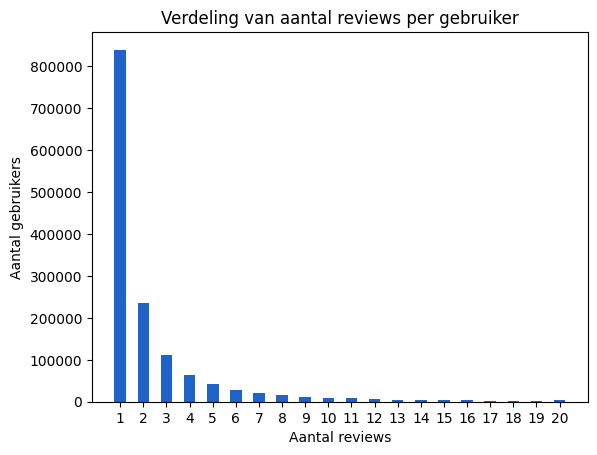
\includegraphics[width=1\linewidth]{fig/chapt3/verdeling_aantal_reviews_per_gebruiker.png}
        \caption{Histogram aantal reviews per gebruiker}
        \label{fig:chapt3_verdeling_aantal_reviews_per_gebruiker}
    \end{subfigure}
    \begin{subfigure}{.5\textwidth}
        \centering
        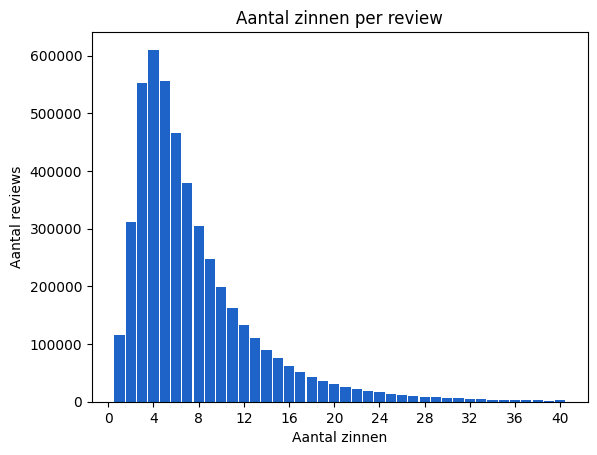
\includegraphics[width=1\linewidth]{fig/chapt3/zin_per_review.png}
        \caption{Histogram aantal zinnen per review}
        \label{fig:chapt3_verdeling_aantal_zinnen_per_review}
    \end{subfigure}
    \caption{Hoeveelheid beschikbare data per gebruiker}
\end{figure}

\subsubsection{Verdeling scores}
De mediaan score over alle gebruikers is 4 van de 5 sterren. De hogere scores komen vaker voor, met 5 de individueel meest voorkomende score.
\begin{figure}[H]
    \begin{subfigure}{.5\textwidth}
        \centering
        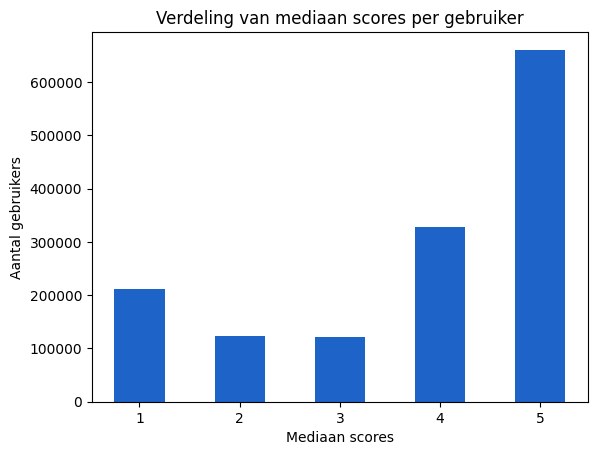
\includegraphics[width=1\linewidth]{fig/chapt3/verdeling_mediaan_scores_per_gebruiker.png}
        \caption{Histogram mediaan reviews per gebruiker}
        \label{fig:chapt3_verdeling_mediaan_scores_per_gebruiker}
    \end{subfigure}
    \begin{subfigure}{.5\textwidth}
        \centering
        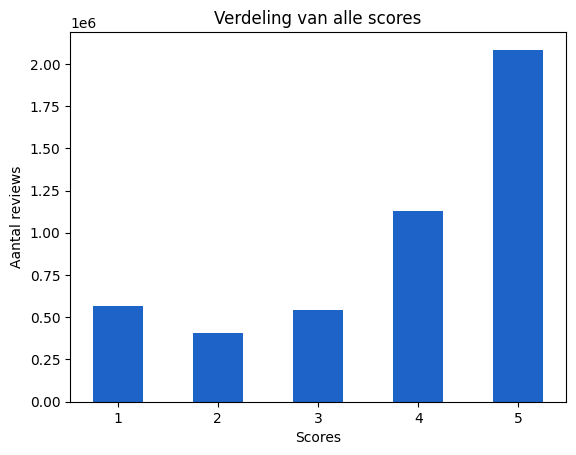
\includegraphics[width=1\linewidth]{fig/chapt3/verdeling_alle_scores.png}
        \caption{Histogram individuele reviews}
        \label{fig:chapt3_verdeling_alle_scores}
    \end{subfigure}
    \caption{Histogrammen over scores}
\end{figure}
We moeten bij de evaluatie van ons aanbevelingssysteem dus rekening houden met deze non-uniforme verdeling. De klassen die lagere scores voorstellen zijn minder vertegenwoordigd in de data, om de gebruikerservaring hoog te houden moeten we voorkomen dat slechte items toch aanbevolen worden.

\subsubsection{Trends binnen dezelfde gebruiker}
De afstand tussen de minimum- en maximumscore die éénzelfde gebruiker geeft is vaak vrij groot. Dit wil zeggen dat gebruikers het volledige spectrum aan scores gebruiken om hun mening uit te drukken. Zelfs wanneer we de meest extra waarden wegfilteren, blijft deze conclusie gelden. Er zijn dus weinig gebruikers die steeds dezelfde score geven. In \autoref{fig:chapt3_verdeling_score_min_max_combined} zijn gebruikers met minder dan 5 reviews weggelaten.
\begin{figure}[H]
    \begin{subfigure}{.5\textwidth}
        \centering
        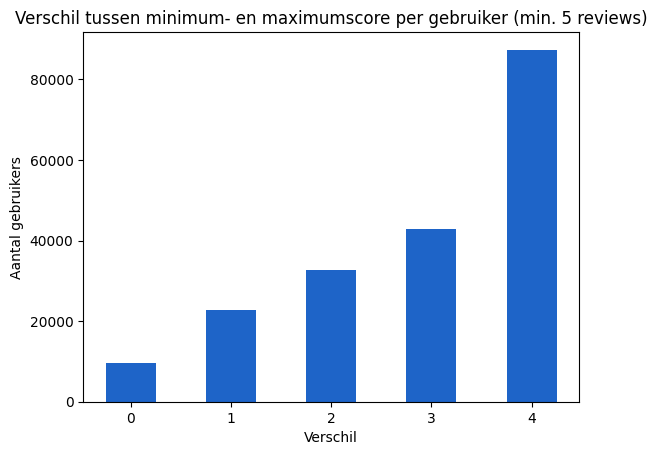
\includegraphics[width=1\linewidth]{fig/chapt3/verdeling_score_min_max.png}
        \caption{Maximumscore - minimumscore}
        \label{fig:chapt3_verdeling_score_min_max}
    \end{subfigure}
    \begin{subfigure}{.5\textwidth}
        \centering
        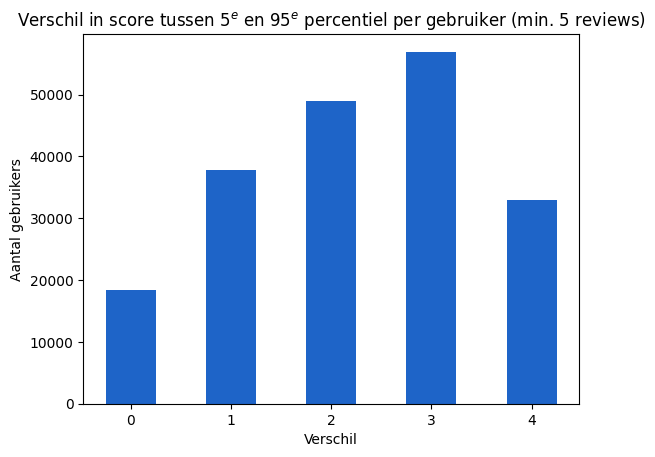
\includegraphics[width=1\linewidth]{fig/chapt3/verdeling_score_min_max_percentiel.png}
        \caption{$95^e$ percentiel - $5^e$ percentiel}
        \label{fig:chapt3_verdeling_score_min_max_percentiel}
    \end{subfigure}
    \caption{Histogrammen over verschil tussen hoge en lage scores binnen dezelfde gebruiker}
    \label{fig:chapt3_verdeling_score_min_max_combined}
\end{figure}

\subsection{Restaurants}
\subsubsection{Reviews per restaurant}
Ieder restaurant uit de dataset heeft minstens 5 reviews van gebruikers. In \autoref{fig:chapt3_verdeling_aantal_reviews_per_restaurant} zijn restaurants met meer dan 155 reviews weggelaten. Merk op dat de dataset veel minder sparse is als we groeperen per restaurant (\ref{sec:chapt3_reviews_per_gebruiker}): weinig gebruikers hebben 5 of meer reviews geschreven, maar ieder restaurant heeft wel minstens 5 reviews. Deze schaarsheid aan reviews per gebruiker suggereert dat IICF beter zal werken op deze dataset dan UUCF. \cite{cursus_hs9}
\mijnfiguur[H]{width=12cm}{fig/chapt3/verdeling_aantal_reviews_per_restaurant.png}{Histogram aantal reviews per restaurant}{fig:chapt3_verdeling_aantal_reviews_per_restaurant}


\subsubsection{Verdeling scores}
De meeste restaurants hebben een mediaan van 4 op 5 sterren. Dit komt op het eerste zicht niet overeen met de bevinding dat de meeste gebruikers een mediaan van 5 op 5 sterren hebben voor hun reviews. Echter blijkt dat de grootste groep van gebruikers met een mediaan van 5 op 5 maar 1 of 2 reviews hebben achtergelaten. We concluderen hieruit dat gebruikers die een groter aantal reviews achterlaten een lagere mediaan hebben.
\mijnfiguur[H]{width=10cm}{fig/chapt3/verdeling_mediaan_scores_per_restaurant.png}{Histogram mediaan reviews per restaurant}{fig:chapt3_verdeling_mediaan_scores_per_restaurant}

\subsubsection{Trends binnen hetzelfde restaurant}
Het verschil tussen de hoogste en laagste score van een restaurant is vaak extreem. Zelfs zonder de 10\% meest extreme scores blijft er een groot verschil. We kunnen hieruit concluderen dat er zeer weinig restaurants bestaan waarvoor alle gebruikers het eens zijn over de score. Dit toont dus aan dat er nood is aan gepersonaliseerde aanbevelingen.
\begin{figure}[H]
    \begin{subfigure}{.5\textwidth}
        \centering
        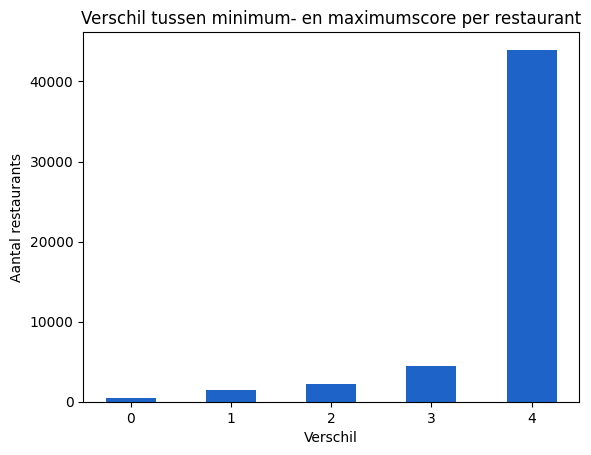
\includegraphics[width=1\linewidth]{fig/chapt3/verdeling_score_min_max_restaurant.png}
        \caption{Maximumscore - minimumscore}
        \label{fig:chapt3_verdeling_score_min_max_restaurant}
    \end{subfigure}
    \begin{subfigure}{.5\textwidth}
        \centering
        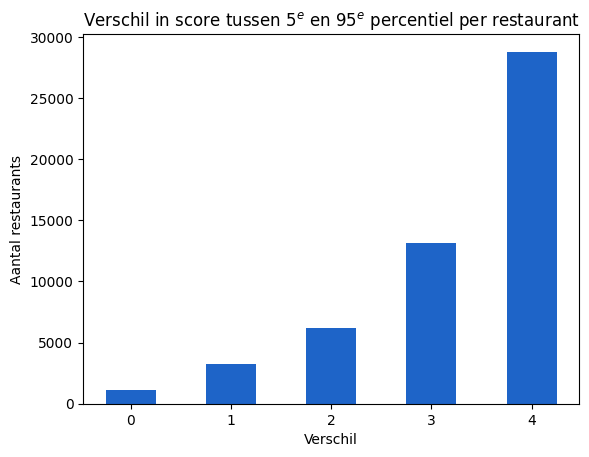
\includegraphics[width=1\linewidth]{fig/chapt3/verdeling_score_min_max_percentiel_restaurant.png}
        \caption{$95^e$ percentiel - $5^e$ percentiel}
        \label{fig:chapt3_verdeling_score_min_max_percentiel_restaurant}
    \end{subfigure}
    \caption{Histogrammen over verschil tussen hoge en lage scores binnen hetzelfde restaurant}
    \label{fig:chapt3_verdeling_score_min_max_combined_restaurants}
\end{figure}
